\section{Method}
\label{sec:method}

\begin{figure*}[t]
\centering
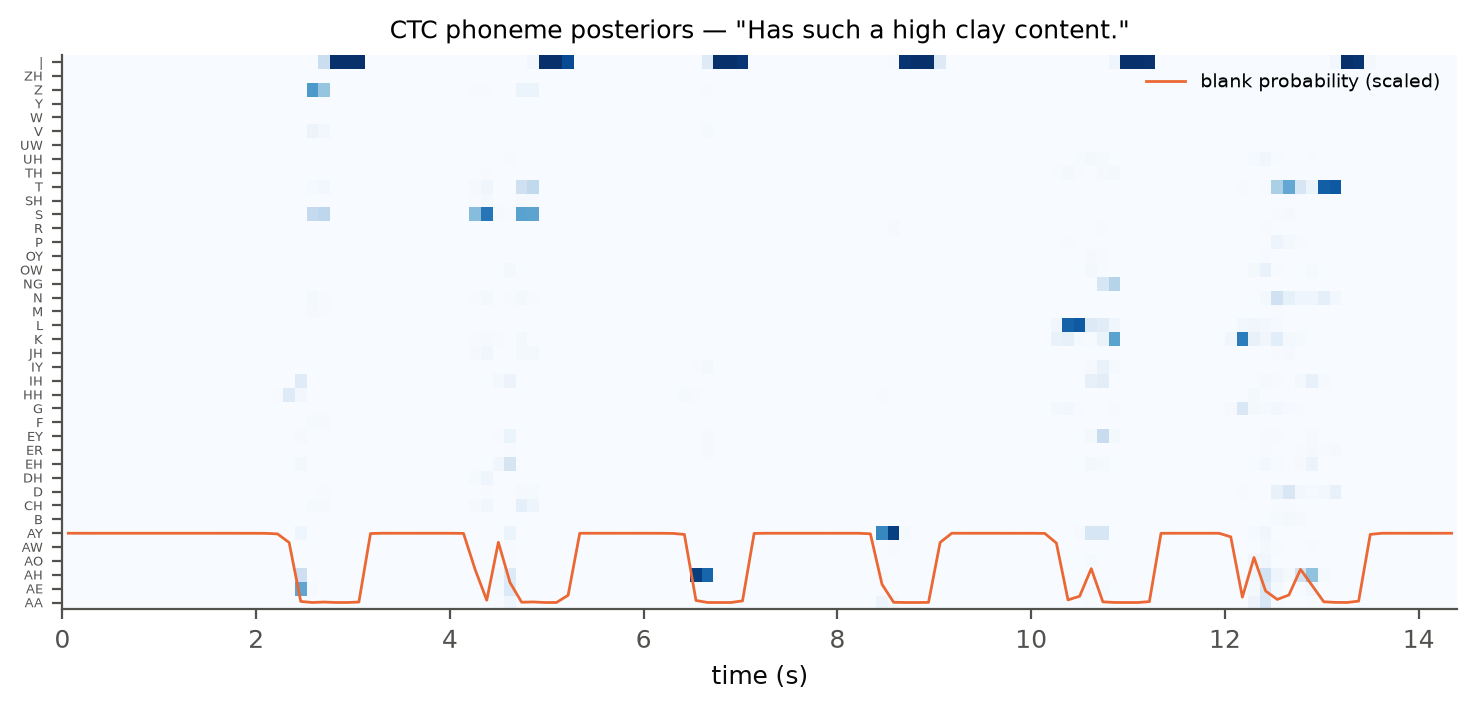
\includegraphics[width=\textwidth]{posteriors_example.png}
\caption{CTC phoneme posteriors of the causal Conformer (seed 0) on a held-out test sentence. Rows are the 39 phonemes plus the word boundary ``$|$''. The orange trace is the blank probability (scaled). The decoder emits sparse, peaky phoneme spikes separated by long blank stretches, typical of CTC. The beam search and LM turn these spikes into words.}
\label{fig:posteriors}
\end{figure*}

\subsection{Problem setup}
A trial gives features $\mathbf{x}_{1:T}\in\mathbb{R}^{T\times 512}$ recorded on day $d$, and a label sequence $\mathbf{y}=(y_1,\dots,y_L)$ over $\mathcal{V}=\{39\text{ phonemes},|\}$. A neural decoder $f_\theta$ outputs frame-level posteriors $p_\theta(k\mid\mathbf{x},t)$ over $\mathcal{V}\cup\{\varnothing\}$ (41 classes) at a reduced frame rate $T'$. Training minimizes the CTC loss
\begin{equation}
\mathcal{L}_{\text{CTC}}=-\frac{1}{L}\log\!\!\sum_{\pi\in\mathcal{B}^{-1}(\mathbf{y})}\prod_{t=1}^{T'}p_\theta(\pi_t\mid\mathbf{x},t),
\end{equation}
where $\mathcal{B}$ collapses repeats and then removes blanks.

\subsection{Shared front end}
\textbf{Day-specific input layers.} Each recording day $d$ has its own affine map, initialized to the identity, followed by a softsign:
$\tilde{\mathbf{x}}_t=\operatorname{softsign}(\mathbf{W}_d\mathbf{x}_t+\mathbf{b}_d)$, with $\mathbf{W}_d\in\mathbb{R}^{512\times512}$ and no weight decay on $\mathbf{W}_d,\mathbf{b}_d$. The ablation \emph{no day layers} shares a single $(\mathbf{W},\mathbf{b})$ across all days.
\textbf{Smoothing and patching.} Features are smoothed with a Gaussian kernel ($\sigma=40$\,ms, matching the published 2 bins of 20\,ms). Windows of $P$ consecutive bins are then concatenated with stride $S$ (``patching''), which sets the output frame rate.
On CPU we average every three consecutive 20\,ms bins into one 60\,ms bin and use $P{=}5$, $S{=}2$: 300\,ms windows every 120\,ms, against 280\,ms every 80\,ms in the published configuration. T15 speaks at about 32 words per minute, and our trials average 1.5 label tokens per second. At 120\,ms per frame that is about 5.5 frames per label, which leaves room for CTC blanks.

\subsection{Baseline: GRU--CTC}
The patched sequence feeds a unidirectional GRU (2 layers, 256 units; published: 5$\times$768) with dropout 0.4 and a linear read-out to 41 classes. GRU input-to-hidden weights use Xavier initialization and hidden-to-hidden weights use orthogonal initialization, as in the released code.
\textbf{Published augmentation} adds white noise ($\sigma{=}1.0$) and a per-trial, per-feature constant offset ($\sigma{=}0.2$), and randomly cuts up to one leading bin.

\subsection{New augmentations: time masking and electrode dropout}
Chronic arrays lose channels over months, and attempted speech is interrupted by pauses and breaths. We add two augmentations, both inspired by SpecAugment \citep{park2019specaugment}.
\emph{Time masking} zeroes up to two spans of up to 480\,ms each.
\emph{Electrode dropout} zeroes \emph{both} features of each electrode independently with probability $q=0.1$, for the whole trial. This simulates an electrode that has failed or gone silent, rather than i.i.d.\ feature noise.
Section~\ref{sec:robust} also uses the same operation as a test-time stressor.

\subsection{Proposed encoder: causal Conformer with self-conditioned CTC}
After the day layers, a per-bin linear bottleneck (512$\to$128) and a patch embedding (Linear+LayerNorm) produce $d{=}144$-dimensional frames. Four Conformer blocks follow \citep{gulati2020conformer}, each a macaron feed-forward $\to$ multi-head self-attention $\to$ convolution module $\to$ feed-forward, with a final LayerNorm. For streaming, attention is causally masked and the depthwise convolution (kernel 15) is left-padded. We use LayerNorm rather than BatchNorm inside the convolution module, so that inference does not depend on batch statistics.
We use no absolute positional encoding: causal masking and the convolutions carry order information. In pilot runs, an unscaled sinusoidal encoding swamped the small patch embeddings.
After block 2 we compute an \emph{intermediate CTC} loss with the shared output head \citep{lee2021intermediate}. Its posteriors are projected back into the residual stream, $\mathbf{h}\leftarrow\mathbf{h}+\mathbf{W}_c\,\mathrm{softmax}(\cdot)$, which is \emph{self-conditioned CTC} \citep{nozaki2021selfcond}. The total loss is $0.7\,\mathcal{L}_{\text{CTC}}+0.3\,\mathcal{L}_{\text{CTC}}^{\text{inter}}$.
A unit test checks causality: perturbing inputs after time $t$ leaves all outputs whose receptive field ends before $t$ unchanged, apart from the 60\,ms half-width of the smoothing kernel.

\subsection{Stabilised CTC training}
\label{sec:stable}
In the previous round of this study, one of two GRU seeds stalled in both GRU configurations and the Conformer spent about 150 steps emitting only blanks. Per-step traces (loss, pre-clip gradient norm and the fraction of frames whose arg\,max is blank; \S\ref{sec:stability}) showed that the stalled seed did \emph{not} suffer exploding gradients: after step 20 its gradient norm stayed near 1, so the clipping threshold of 10 was never reached. Instead, its first $\sim$20 steps were spent learning to emit blanks from a uniform initial posterior (initial loss $\approx$16, gradient norms up to 13 during warm-up), after which it sat on the ``blank plus frequent phonemes'' plateau that CTC models are known to pass through \citep{zeyer2021peaky}. We changed five things, all standard:
(i)~\textbf{blank-logit initialisation}: the read-out bias of the blank starts at $b{=}4$, so $p(\varnothing)=e^{b}/(e^{b}+40)=0.58$, close to the frame-level blank rate of a trained model, and the first updates go to the label logits;
(ii)~\textbf{input re-standardisation}: averaging three z-scored 20\,ms bins shrinks the feature s.d.\ to 0.63, so the published white-noise augmentation ($\sigma{=}1$, set for unit-variance inputs) had a 1.6$\times$ lower signal-to-noise ratio than intended; we rescale the binned features by one global constant (1/s.d.\ of the training features);
(iii)~\textbf{a short-utterance curriculum} for the first 100 steps (the shorter half of the training sentences), in the spirit of SortaGrad \citep{amodei2016deepspeech2};
(iv)~\textbf{a longer linear warm-up} (100 steps instead of 50) before the cosine decay \citep{loshchilov2017sgdr}; and
(v)~\textbf{gradient-norm clipping at 1} instead of 10 \citep{pascanu2013difficulty}, so that the rare large steps are bounded.
The Conformer keeps its intermediate, self-conditioned CTC loss, which also acts as an auxiliary signal for the lower blocks.

\subsection{Ensembling}
Following the Brain-to-Text~'24 lessons, we ensemble models of the same architecture trained with different seeds by averaging their per-frame posteriors, $\bar p(k\mid t)=\tfrac1M\sum_m p_{\theta_m}(k\mid t)$, and then decode $\bar p$.

\subsection{Phoneme-to-word decoding}
\textbf{Lexicon and LM.} The vocabulary is every word with a CMUdict pronunciation \citep{cmudict} that occurs at least twice in the LM corpus or appears in a training cue sentence: \LMVocab{} words, with \LMOOV\% out-of-vocabulary tokens on the evaluation sentences.
The corpus is OpenWebText-10k \citep{gokaslan2019openwebtext}, DailyDialog \citep{li2017dailydialog} and the cue sentences of the training trials, \LMWords\,M words in total. Any corpus sentence that matches a dev or test sentence after normalization is removed (\LMRemoved{} sentences).
We fit an interpolated Kneser--Ney trigram \citep{kneser1995improved,chen1999empirical} with discount $D{=}0.75$ (\LMTrigrams\,M trigrams). It is stored as sorted 64-bit keys and queried by binary search.

\textbf{Beam search.} Hypotheses walk a phoneme trie of the vocabulary under the CTC prefix recursion \citep{hannun2014firstpass}. When the decoder emits ``$|$'' at a trie node where one or more words end, the hypothesis commits each such word (homophones branch). Each committed word $w$ adds
\begin{equation}
\alpha\log P_{\text{KN}}(w\mid w_{-2},w_{-1})+\beta
\end{equation}
to the hypothesis score. A hypothesis that ends inside a word is completed or dropped, and the score for the end-of-sentence token is then added. We use beam 32. Frames with blank probability above 0.999 are skipped, and tokens with log-probability below $-8$ are pruned.
\emph{No-LM} decoding uses the same lexicon-constrained search with $\alpha{=}0$.

\textbf{LLM rescoring.} The 10-best list is rescored with
\begin{equation}
s=\log p_{\text{CTC}}+\alpha\log P_{\text{KN}}+\beta|w|+\gamma\log P_{\text{GPT-2}},
\end{equation}
where GPT-2 small (124M parameters; \citealp{radford2019gpt2}) stands in for the 6.7B-parameter OPT used clinically.
\textbf{Tuning on dev only.} All decoder settings are chosen on the 215 dev sentences (held-out trials of the training sessions, disjoint from the 426 test sentences), separately for each system, and the test set is then decoded once. The lexicon-only word bonus is searched first; $(\alpha,\beta)$ by two rounds of coordinate descent; then the beam width (8--64, ceiling 128); finally $\gamma$ jointly with a re-tuned word bonus on the dev 10-best lists. Every one-dimensional search starts from a grid and, whenever the optimum falls on an edge, extends the grid past that edge (multiplicatively for $\alpha$, $\gamma$ and the beam, additively for the bonuses) until the optimum is interior or a hard bound is reached ($\gamma\ge0$, beam $\le128$).

\subsection{Unsupervised adaptation to a new day}
\label{sec:tta}
For a new session we change only that day's input layer $(\mathbf{W}_d,\mathbf{b}_d)$, initialised from the most recent training day's layer, and use only \emph{unlabelled} neural data from the new day (its \texttt{train} split; never the test sentences).
\textbf{Feature-statistics matching} maps the new day's features onto the statistics of the most recent training day by an affine map $\mathbf{x}\mapsto\mathbf{x}\mathbf{A}+\mathbf{c}$ and folds it into the copied layer ($\mathbf{W}_d\leftarrow\mathbf{A}\mathbf{W}_{d-1}$, $\mathbf{b}_d\leftarrow\mathbf{c}\mathbf{W}_{d-1}+\mathbf{b}_{d-1}$). We use either per-feature mean/s.d.\ matching or CORAL \citep{sun2016coral}, $\mathbf{A}=\mathbf{C}_{\text{new}}^{-1/2}\mathbf{C}_{\text{ref}}^{1/2}$, with 10\% shrinkage of each covariance toward its diagonal.
\textbf{Self-training} \citep{kahn2020selftraining}, close in spirit to the LM-corrected self-recalibration of \citet{fan2023plug}: the unlabelled sentences are decoded with the lexicon + trigram beam search, the decoded words are turned back into phoneme targets with the pronunciation lexicon, and the half of the sentences whose greedy phoneme string agrees least with that pseudo-label (1\,$-$\,PER between the two) is discarded. The day layer is then fine-tuned with CTC on the rest for 40 steps, exactly as in supervised calibration, and the procedure is repeated for two rounds. We also run self-training starting from the CORAL-initialised layer.
